%%%%%%%%%%%%%%%%%%%%%%%%%%%%%%%%%%%%%%%%%%%%%%%%%%%%%%%%%%%%
%%%  Augmenting TV Newscasts via Entity Expansion  %%%
%%%%%%%%%%%%%%%%%%%%%%%%%%%%%%%%%%%%%%%%%%%%%%%%%%%%%%%%%%%%

\documentclass{llncs}

\newcommand{\superscript}[1]{\ensuremath{^{\textrm{#1}}}}

\usepackage{makeidx}  % allows for indexgeneration
\usepackage[hyphens]{url}
\usepackage{textcomp}
\usepackage{color}
\usepackage{listings}
\usepackage{multirow}
\usepackage{mathtools}
\usepackage{graphicx}
\usepackage{fancyvrb}
\usepackage{amsmath}
\usepackage{graphicx}
\usepackage[font=small,labelfont=bf]{caption}
\setcounter{MaxMatrixCols}{20}
\usepackage{pbox}
\usepackage{amsfonts}


% listing styles
\lstset{numbers=left, numberstyle=\tiny,basicstyle=\ttfamily\scriptsize, tabsize=2, keywordstyle=\underbar, stringstyle=\small, backgroundcolor=\color[gray]{0.94}, framexleftmargin=2pt}
\lstdefinestyle{rdfa}{numberblanklines=true, morekeywords={}}



\begin{document}
\frontmatter          % for the preliminaries
\pagestyle{headings}  % switches on printing of running heads
\mainmatter              % start of the contributions

\title{Augmenting TV Newscasts via Entity Expansion}
\author{Jos\'e Luis Redondo Garc\'ia\inst{2}, Michiel Hildebrand\inst{1}, Lilia Perez Romero\inst{1}, Rapha\"el Troncy\inst{2}}
\institute{CWI, Amsterdam, The Netherlands, \\
\email{\{M.Hildebrand, L.Perez\}@cwi.nl}
\and
EURECOM, Sophia Antipolis, France, \\
\email{\{redondo, raphael.troncy\}@eurecom.fr}
}


\maketitle              % typeset the title of the contribution

%%%%%%%%%%%%%%%%%%
%%%  Abstract  %%%
%%%%%%%%%%%%%%%%%%

\begin{abstract}
The presence of appropriate TV content annotations and usage of custom visualization strategies are key factors to enhance the viewer experience. In this paper, we present an approach that leverages on the knowledge present on the Web for identifying and enriching relevant items inside a News video and displaying them in a timely and user friendly fashion. 
In particular, this second screen prototype (i) collects and offers information about persons, locations, organizations and concepts occurring in the newscast, and (ii) combines them for enriching the underlying story along five main dimensions: in other sources, expert's opinions, timeline of the news, in depth information, and geo-localized comments and remarks from other viewers.  
Starting from preliminary insights coming from the named entities spotted on the video subtitles, we expand this initial context to a broader event representation by relying in the knowledge of other non-structured Web documents talking about the same fact. This makes possible to generate a much richer, context aware metadata of a TV program that boost the viewer interaction and opens new possibilities in the hyperlinked television domain. 

\keywords{Multimedia Annotation, Entity Expansion, Newscast Enrichment}
\end{abstract}

%%%%%%%%%%%%%%%%%%%%%%%%%
%%%  1. Introduction  %%%
%%%%%%%%%%%%%%%%%%%%%%%%%

\section{Introduction}

People consume news from multiple sources, such as television, Web, radio and newspaper. For example, we watch the newscast on TV early in the morning to get an overview of the main news, we use the Web to keep track of the News throughout the day, and when we have some spare time we actively browse the Web to explore the news items that we are interested in. At the end of the day, our understanding about the news is a compendium of various information pieces coming from different sources, which complement each other and enrich our news experience. The problem is that in practice it is difficult and time consuming to manually gather all those insights together. Our research tackles this inconvenience by quickly offering extra information about the newscast organized in various dimensions which intend to illustrate all those details you watched but would like to further explore. 

%News Prototypes
There are already some approaches that address this content augmentation of news broadcasts, like the work done by Dowman et al.~\cite{DowmanEtAl05c}. Their system identifies individual stories in news broadcasts and annotates them with content from the World Wide Web. Annotations are used to produce summarized texts that can be employed potentially for enrichment of electronic program guides. Even this is a first step through the integration of television newscasts with Web content, it does not trust completely in automatic processes for providing a user centric news consumption and delegates on an interface for the postproduction (curating and editing) phase of the enriched hypermedia. Regarding the technical aspect the we opted for a Second screen multitasking schema, a growing practice that has triggered the interest of industry and stimulated the proliferation of commercial applications for dual device set- ups. One of the best known examples is Yahoo�s IntoNow~\footnote{\fontsize{8pt}{1em}\selectfont \url{http://www.intonow.com/ci}}, which uses audio fingerprinting technology to automatically detect the program that users are watching and deliver related contents. 

% Semantic
The problem of multimedia annotation has been traditionally addressed by applying different analysis techniques~\cite{ballan2011event}, but extracting semantic information from a video is still a challenging task. One possible approach consists in using Named Entity Recognition (NER) over the textual information attached to particular video fragment. Those techniques are an essential component within the Information Extraction field that focus on: identifying atomic information units in texts, named entities; classifying entities into predefined categories (also called context types) and linking to real world objects using web identifiers (Named Entity Disambiguation). A growing number of APIs provide such a service, like AlchemyAPI\footnote{\fontsize{8pt}{1em}\selectfont \url{http://www.alchemyapi.com/}} or DBpedia Spotlight\footnote{\fontsize{8pt}{1em}\selectfont \url{http://spotlight.dbpedia.org/}}. If the textual information attached to a video contains temporal references (e.g. subtitles), it is possible to align the entities with the time when they appear in the video. Katsiouli et al.~\cite{katsiouli2007} have demonstrated that applying named entity recognition techniques in combination with domain ontologies on video subtitles can produce good results for video classification. Other entity based annotation tool has been proposed by Yunjia et al.~\cite{yunjia2013} also relies in name entity recognition techniques for finding relevant concepts within the video fragments. 

% SecondScreen

%%%%%%%%%%%%%%%%%%%%%%%%%%
%%%  Augmenting and Enriching TV News    %%%
%%%%%%%%%%%%%%%%%%%%%%%%%%

\section{Augmenting and Enriching TV News}
\label{sec:tvnews}

LinkedTV News is a second screen application for tablets that acts as a companion to viewers when watching the news broadcasts. Its main goal is to enrich television newscasts by integrating them with other media thus. It is designed to accommodate two viewing modes in terms of interaction: a lean back mode and a lean forward mode. 

\begin{figure}[h!]
\centering
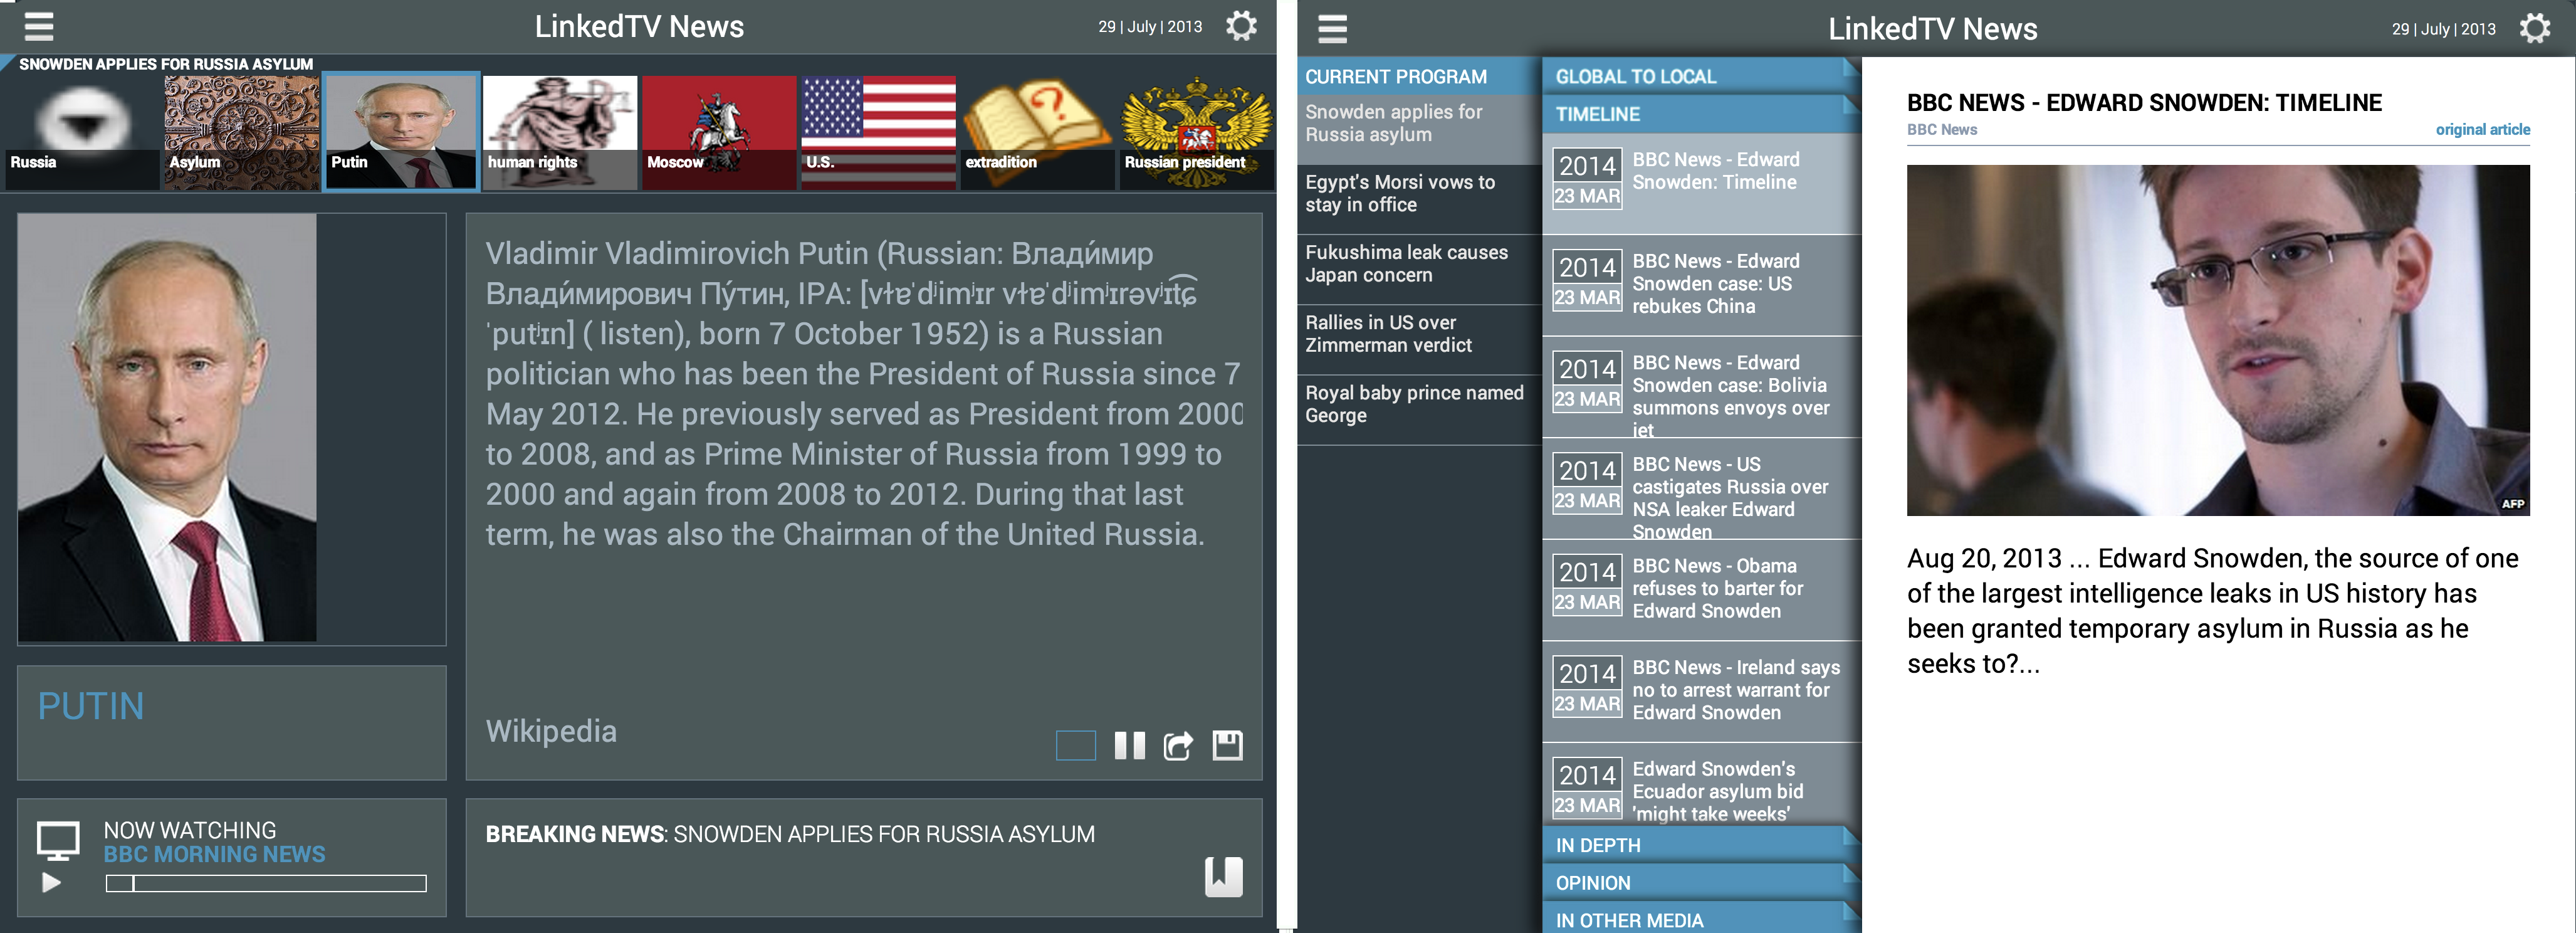
\includegraphics[width=1\textwidth]{figure/DemoScreen}
\caption{Demo screen captures corresponding to the (1) active mode and the (2) passive mode.}
\label{fig:namedEntityExpansion}%\end{figure}
\end{figure}

In the passive mode the application operates as a second screen that is synced with the TV program. This mode supports the user with looking up factual information by presenting timed slides about the entities that occur in the news. As this mode requires no interaction it unobtrusively complements the lean back TV viewing experience. In addition, the passive mode provides functionality to bookmark news items. This one click interaction forms the bridge to the active mode of the application. 

In the active mode the user actively explores a specific news item. In this mode the application contains articles from the Web that are related to the news item in different dimensions. The dimension, such as articles from different news sources, opinion articles and a timeline of past events, are intended to support the specific user information needs that were identified in the study. While it is possible to use the active mode during the broadcast, this will disrupt the passive TV viewing experience. By first bookmarking the news item the user can come back to the application at a more appropriate time to start or continue the exploration.

The application LinkedTV News synchronizes its content automatically with the television without any action required from the users. 

IN the following sections we will give the details:

%%%  The Lean-back Mode  %%%
\subsection{The Lean-back Mode}
\label{sec:leanbackmode}

Requires minimum interaction. The main elements and information about them.
In this mode, the application presents the user with summarized additional information about elements of the news, for example, basic information about the location or people involved. This happens in the form of a slideshow with short texts and images that acts as a sort of news ticker to the broadcast appearing in the main screen. It automatically synchronizes with the TV, and requires no action from the user, but allows the user to browse slides, save them or bookmark news for later exploration. This lean back mode of the application intends to be as close as possible to a free hand, and passive experience. The slides are presented without need for user interaction, so the user can relax, share with her company and pay attention only to that which really calls her interest while easily bookmarking her favorite news for later reading. This favors an asynchronous mode of interaction that respects a passive mode of TV watching, and allows postponing the more attention demanding activities by using the TV program as an index for deciding what to explore in a more suitable time.

To reconstruct the semantic context associated with one particular news video, we extract the main concepts and entities from the subtitles and explain how they are related to each other. The complete processing workflow takes as input the textual transcript of a multimedia resource illustrating an event, as well as the start and end date for which that particular event is considered. We assume that this event has a minimal presence and coverage on the Web to ensure that the subsequent data mining techniques can collect sufficient data to reconstruct the event's context. 

For each news item, we perform named-entity recognition over the corresponding subtitles using the NERD framework~\cite{Rizzo2012b}. In our experiment, the language of the videos is English but NERD supports other languages. The output of this phase is a collection of entities annotated using the NERD Ontology\footnote{\fontsize{8pt}{1em}\selectfont \url{http://nerd.eurecom.fr/ontology/nerd-v0.5.n3}}, that comes with a first relevance score obtained from the extractors which have been used. This set includes a list of ranked entities that are explicitly mentioned during the video. Other entity based video annotation tools~\cite{yunjia2013} stop at this point even when entities that can be relevant for the viewer in the context of the event are still missing. We tackle this problem by extending this first list of concepts via the entity expansion component.

The set of entities obtained from a traditional named entity extraction operation is normally insufficient and incomplete for expressing the context of a news event. Sometimes, some entities spotted over a particular document are not disambiguated because the textual clues surrounding the entity are not precise enough for the name entity extractor, while in other cases, they are simply not mentioned in the transcripts while being relevant for understanding the story. We perform the a process named entity expansion operation, which relies on the idea of retrieving and analyzing additional documents from the Web where the same event is also described. By increasing the size of set of documents to analyse, we increase the completeness of the context and the representativeness of the list of entities, reinforcing relevant entities and finding new ones that are potentially interesting inside the context of that news item.

The entire logic is illustrated in in Figure~\ref{fig:namedEntityExpansion} and consists mainly in (1) building an appropriate search query from the original set of entities, (2) retrieving additional documents about the same news event, and (3) analyzing them for providing a more complete and better ranked set of final entities, as illustrated in Figure~\ref{fig:namedEntityExpansion}.

\begin{figure}[h!]
\centering
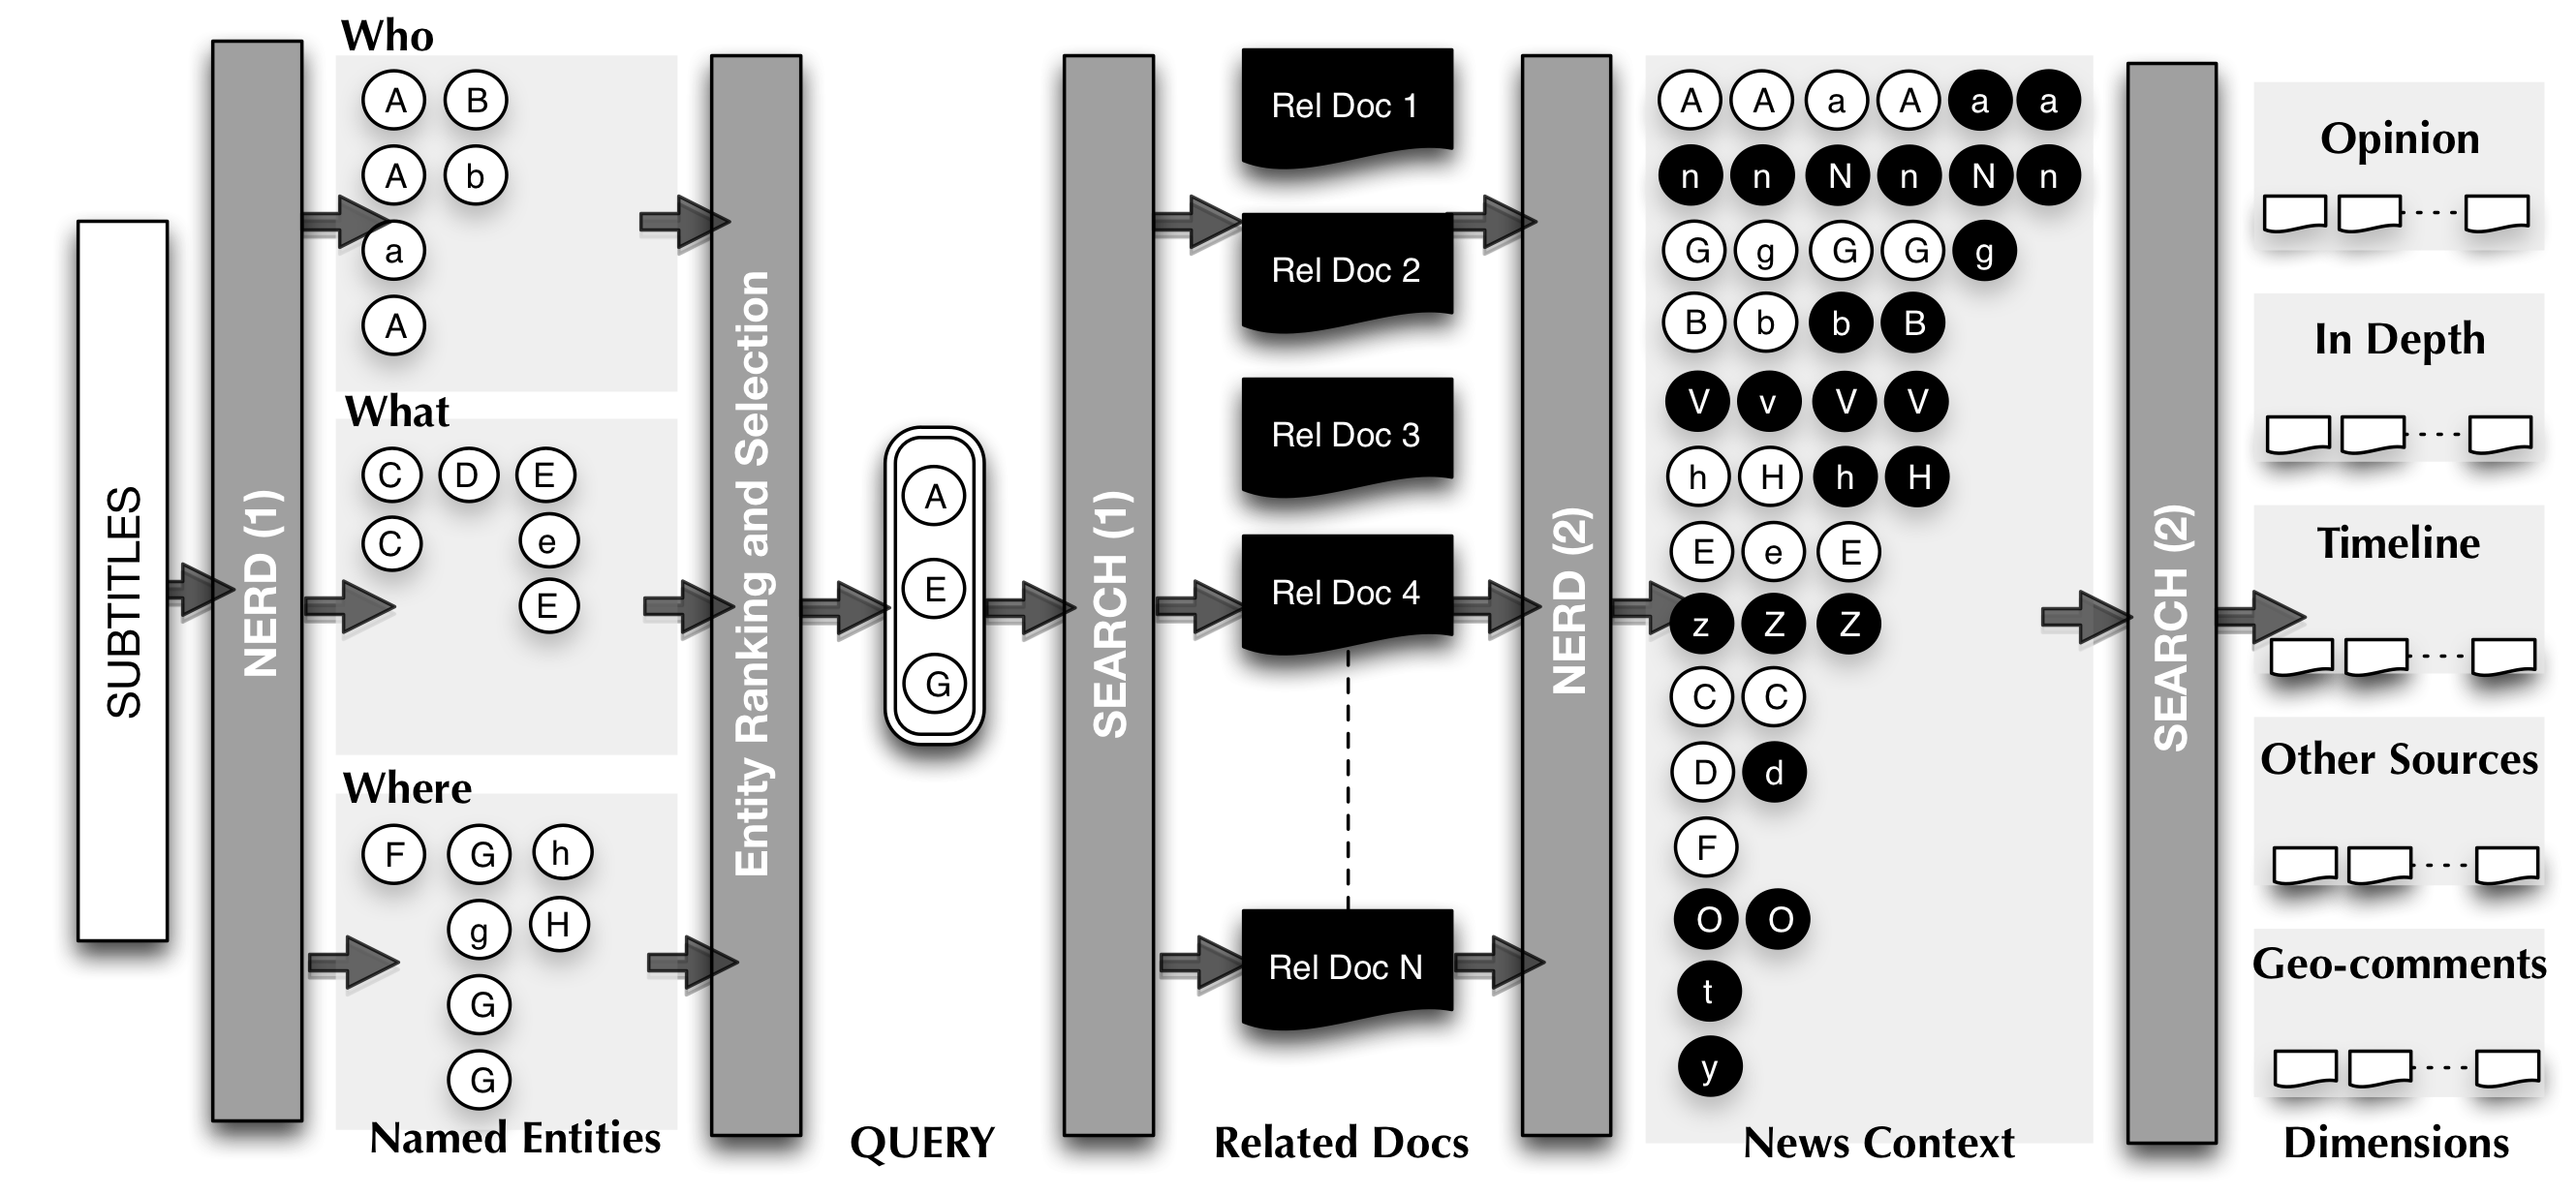
\includegraphics[width=1\textwidth]{figure/ExpansionDiagram}
\caption{Schema of Named Entity Expansion Algorithm.}
\label{fig:namedEntityExpansion}%\end{figure}
\end{figure}

\subsubsection{Query Generation}
\label{sec:querygeneration}
The \emph{Five W's} is a popular concept of information gathering in journalistic reporting. It captures the main aspects of a story: who, when, what, where, and why~\cite{LiJia2007}. We try to represent the news item in terms of four of those five W's (who is involved in the event, where the event is taking place, what the event is about, and when it has happened) in order to generate a query that retrieves documents associated to the same event.

First, the original entities are mapped to the NERD Core ontology, which considers 10 main classes: Thing, Amount, Animal, Event, Function, Organization, Location, Person, Product and Time. From those ten different categories, we generalize to three classes: the Who from \url{nerd:Person} and \url{nerd:Organization}, the Where from \url{nerd:Location}, and the What from the rest of NERD types after discarding \url{nerd:Time} and \url{nerd:Amount}. The When or so-called temporal dimension does not need to be computed since it is considered to be provided by the video publisher.

After generating the three sets of entities, the next step consist in ranking them in relevance according to a weighted sum of two different dimensions: their frequency in the transcripts and their former relevance scores coming from the named entity extractors. We have defined the function \emph{filterEntities(S)} for selecting the $n$ entities inside the set of entities $S$ whose relative relevance falls into the upper quarter of the interval.

The final query is a pair where \textit{textQuery} is the result of concatenating the labels of the most relevant entities in the sets Who, What, Where in that particular order, and $t$ the time period dimension. This query generation is depicted in the upper part of Figure~\ref{fig:namedEntityExpansion}.

\subsubsection{Document Retrieval}
Once $\text{Query}_{Event}$ is built out of the original set of named entities, it will be ready to be injected into a document search engine where additional descriptions about the news event can be found. In this situation, the kind of query generated in the previous step and the search engine chosen should be closely tied in order to maximize the quality of the obtained results. The different behavior of search engines make some alternatives more suitable than others for certain kinds of events. The way the resulting documents change in the search engines for a particular kind of event is a research question that will not be studied in this paper.

In this paper, we rely on the Google Search REST API service\footnote{\fontsize{8pt}{1em}\selectfont  \url{http://ajax.googleapis.com/ajax/services/search/web?v=1.0}} by launching a query with the text \textit{textQuery}. Due to quota restrictions imposed by Google, the maximum number of retrieved document is set to 30. However, as shown in the evaluation described in the Section~\ref{sec:evaluation}, this is enough for significantly extending the initial set of entities directly spotted by NERD.

Concerning the temporal dimension, we only keep the documents published in the time period $t+t_{e}$. We increase the original event period in $t_{e}$ because documents concerning a news event are not always published during the time of the action is taking place but some hours or days after. The value of $t_{e}$ depends on many factors such as the nature of the event itself (whether it is a brief appearance in a media, or part of a longer story with more repercussion) or the kind of documents the search engine is indexing (from very deep and elaborated documents that need time to be published, to short post quickly generated by users). Based on the simple assumption that that the longer is an event, and the longer it is likely to generate buzzes, we approximated  $t_{e} = t$ which means that we also consider document published during the course of an event.

The middle part of Figure~\ref{fig:namedEntityExpansion} shows this process. The query is input in the search engine in order to retrieve other documents that report on the same event discussed in the original video. Those documents (colored in black in the Figure~\ref{fig:namedEntityExpansion}) will be further processed to increase the size of the collection and get additional insights about the news item.

\subsubsection{Entity Clustering}
In this phase, the additional documents which have just been retrieved are now processed and analyzed in order to extend and re-rank the original set of entities and consequently get a better insight about the event. Since most of the resources retrieved are Web pages, HTML tags and other annotations are removed, keeping only the main textual information. This plain text is then analyzed by the NERD framework in order to extract more named entities.

In order to calculate the frequency of a particular resource within the entire corpora, we group the different appearances of the same instance and check their cardinality. This is not a trivial task since the same entity can appear under different text labels, contain typos or have different disambiguation URL's pointing to the same resource. We performed a centroid-based clustering operation over the instances of the entities. We considered the centroid of a cluster as the entity with the most frequent disambiguation URL's that also have the most repeated labels. As distance metric for comparing pairs of entities, we applied strict string similarity over the URL's, and in case of mismatch, the Jaro-Winkler string distance~\cite{winkler2006overview} over the labels. The output of this phase is a list of clusters containing different instances of the same entity.

\subsubsection{Entity Ranking}
The final step of the expansion consists of ranking the different named entities obtained so far. To create this ordered list, we assigned a score to every entity according to the following features: relative frequency in the transcripts of the event video; relative frequency over the additional document; and average relevance according to the named entity extractors. The three dimensions are combined via a weighted sum where the frequency in the video subtitles has a bigger impact, followed by the frequency on the searched documents and the relevance from the extractors. The final output of the entity expansion operation is a list of entities together with their ranking score and the frequency in both the main video and in the collected documents retrieved from the search engine.

Entities with a higher $relScore_{i}$ in the final classification are considered more representative for describing the context than the original entities. 


%%%  The Lean-Forward Mode %%%
\subsection{The Active Mode}
\label{sec:leanforwardmode}

The active mode of the application acts as a hub where the viewers can access extra documents for complementing what is being told in the main news video. A similar logic to the one explained in Section~\ref{sec:querygeneration} is applied over the main entities coming from the expansion process for building custom queries in Google CSE, but relaxing or emphasizing some particular \emph{W's} and operating over particular lists of Web resources. In contrast to traditional news aggregators that simply gather related documents, the results are organized around five different axes that intent to fulfill the viewer' needs. 

\textbf{Timeline.} Follows the news story throughout time by confectioning an list of ordered documents that includes the main antecedents of the present facts. For getting those document we rely on a query without any prior time constraint, which is created when including the most relevant entity from the Who, Was, Where inside the pattern ''The'' + entity + "case". For our example we have obtained the text "The Edward Snowden case".

\textbf{In other sources.} This section of the interface is dedicated to showing the selected news as it was reported in other newspapers, radio, or TV programs. We launch a query generated from the set of expanded entities by following exactly the same logic in Section~\ref{sec:querygeneration}, over a curated list of resources including mainly Journals and television broadcasters Web sites. In our example the query looks like "Asylum Edward Snowden Russia"

\textbf{Opinion.} This section is devoted to gathering opinions regarding the selected news item from different authors with a certain presupposed knowledge about the matter. The list of documents is obtained by executing the same query generated for dimension ''In other Sources'', but operating over a different list of curated resources that considers only subdomains specialized in opinion documents.

\textbf{Geo-localized information.} This section includes live feeds from Twitter expressing people�s remarks, comments and feelings filtered by subject and geo-location. We use the same query built for the dimension ''In other Sources'', but reducing the temporal dimension $t$ to the last 7 days from the current time in order to see what the people is thinking about the particular news item.

\textbf{In depth.} Includes in depth coverage articles that offer a more extensive view about the seed news item. They documents under this dimension are obtained by combining the most relevant entity from the Who, Was, Where with the keyword "in depth" and removing any temporal restriction and extending the search domain to the entire Web. In our example the textual will be "Edward Snowden in depth";
		
%%%%%%%%%%%%%%%%%%%%%%%
%%%  4. Discussion  %%%
%%%%%%%%%%%%%%%%%%%%%%%

\section{Discussion}
\label{sec:discussion}
The preliminary results indicate that we are able to offer to the viewer a relevant set of entities that expands the initial concepts detected by traditional named entity recognition approaches and covers a wider range of user information needs. Many details not explicitly mentioned in the video but important in the context of the newscasts are now available to the viewer to be consumed, either during he is watching the news (passive mode) or when he browses additional insights (active mode).

At the same time those detected concepts are used as powerful triggers for detecting extra knowledge from the Web along 5 main dimensions. Some of those axes are focused on providing the big picture of the news event (\emph{timeline} and \emph{in depth}). Others are intended to help the viewer to corroborate the facts in alternative sources (\emph{In other sources}) and obtain feedback from professionals and journalists (\emph{opinion}). Finally, keeping in mind that TV newscasts viewing is a potentially social activity, one of the dimensions include live feeds from twitter filtered by subject and by geo-location. 

In the future we plan to continue improving the way detected concepts are ranked in relevance and therefore chosen as candidates for answering particular viewer's demands or trigger new enrichments. We also look forward to a more exhaustive evaluation based on viewers' feedback from surveys and open interviews where we can gather more information about which are the viewer's requirements to potentially fulfill the aimed hypervideo experience.

%%%%%%%%%%%%%%%%%%%%%%%%%
%%%  Acknowledgments  %%%
%%%%%%%%%%%%%%%%%%%%%%%%%

\section*{Acknowledgments}
This work was partially supported by the European Union's 7th Framework Programme via the project LinkedTV (GA 287911).

%%%%%%%%%%%%%%%%%%%%%%
%%%  Bibliography  %%%
%%%%%%%%%%%%%%%%%%%%%%
\bibliographystyle{abbrv}
\bibliography{EnrichedTVNews}

\end{document}
